\documentclass[UTF8]{article}
\usepackage{graphicx}
\usepackage{subfigure}
\usepackage{amsmath}
\usepackage{makecell}
\usepackage[utf8]{inputenc}
\usepackage[space]{ctex} %中文包
\usepackage{listings} %放代码
\usepackage{xcolor} %代码着色宏包
\usepackage{CJK} %显示中文宏包
\usepackage{float}

\definecolor{mygreen}{rgb}{0,0.6,0}
\definecolor{mygray}{rgb}{0.5,0.5,0.5}
\definecolor{mymauve}{rgb}{0.58,0,0.82}
\lstset{
	backgroundcolor=\color{white}, 
	basicstyle = \footnotesize,       
	breakatwhitespace = false,        
	breaklines = true,                 
	captionpos = b,                    
	commentstyle = \color{mygreen}\bfseries,
	extendedchars = false,
	frame = shadowbox, 
	framerule=0.5pt,
	keepspaces=true,
	keywordstyle=\color{blue}\bfseries, % keyword style
	language = C++,                     % the language of code
	otherkeywords={string}, 
	numbers=left, 
	numbersep=5pt,
	numberstyle=\tiny\color{mygray},
	rulecolor=\color{black},         
	showspaces=false,  
	showstringspaces=false, 
	showtabs=false,    
	stepnumber=1,         
	stringstyle=\color{mymauve},        % string literal style
	tabsize=4,          
	title=\lstname           
}


%画图包
\usepackage{tikz}
%画图背景包
\usetikzlibrary{backgrounds}

%自定义命令
\newcommand{\psiG}{\psi_{G}}
%在tikz中画一个顶点
%#1:node名称
%#2:位置
%#3:标签
\newcommand{\newVertex}[3]{\node[circle, draw=black, line width=1pt, scale=0.8] (#1) at #2{#3}}
%在tikz中画一条边
\newcommand{\newEdge}[2]{\draw [black,very thick](#1)--(#2)}
%在tikz中放一个标签
%#1:名称
%#2:位置
%#3:标签内容
\newcommand{\newLabel}[3]{\node[line width=1pt] (#1) at #2{#3}}
\newcommand{\jumpLine} {\hspace*{\fill} \\}


\title{中国科学技术大学计算机学院\\《数据结构》报告}
\author{}
\date{}

\begin{document}
\maketitle
	\begin{figure}[H]
		\centering
		
\includegraphics[width=2.5in]{xiaohui.jpg}\vspace{0.5cm}\\
		\large{
			实验题目:二叉树及其应用\\
			学生姓名:王章瀚\\
			学生学号:PB18111697\\
			完成日期:\today\\
		}\vspace{2cm}
		
		\large{计算机实验教学中心制\\2019年09月\\}
		\thispagestyle{empty}
		\clearpage  % 清除当页页码
	\end{figure}
	\newpage
	
	\section{实验要求}
	本次实验分为两个小实验。\par
	\subsection{二叉树的创建与遍历}
	\textbf{概述}\par
	通过添加虚结点,为二叉树的每一实结点补足其孩子,再对补足虚结点后的二叉树按层次遍历的次序输
	入。\par
	例如:ABC\#DEFG\#\#H\#\#\#\#\#\#\par
	\begin{figure}[H]
		\centering
		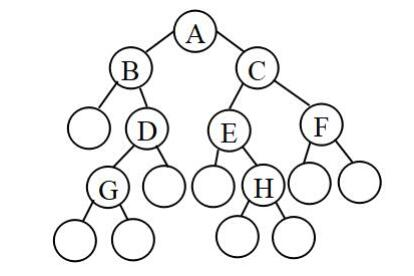
\includegraphics[width=0.6\linewidth]{sampleTree.jpg}
		\label{sampleTree}
	\end{figure}\par
	构建这颗二叉树(不包含图中的虚结点),并增加左右标志域,将二叉树后序线索化\par
	完成后序线索化树上的遍历算法,依次输出该二叉树先序遍历、中序遍历和后序遍历的结果。\par
	
	\textbf{输入与输出}\par
	样例如下:\par
	\fbox{
		\parbox{0.8\linewidth}{
			Input:\\
			ABC\#DEFG\#\#H\#\#\#\#\#\#\\
			output:\\
			ABDGCEHF\\
			BGDAEHCF\\
			GDBHEFCA\\
		}
	}\par
	
	\subsection{表达式树}
	\textbf{概述}\par
	输入合法的波兰式(仅考虑运算符为双目运算符的情况),构建表达式树,分别输出对应的中缀表达式(可含有多余的括号)、逆波兰式和表达式的值,输入的运算符与操作数之间会用空格隔开。\par
	构建这颗二叉树(不包含图中的虚结点),并增加左右标志域,将二叉树后序线索化\par
	完成后序线索化树上的遍历算法,依次输出该二叉树先序遍历、中序遍历和后序遍历的结果。\par
	
	\textbf{输入与输出}\par
	样例如下:\par
	\fbox{
		\parbox{0.8\linewidth}{
			Input:\\
			- + 2 3 1 //波兰式\\
			Output:\\
			(2+3)-1 //中缀表达式\\
			2 3 + 1 - //逆波兰式\\
			4 //求值\\
		}
	}\par
	对应表达式树如下:\par
	\begin{figure}[H]
		\centering
		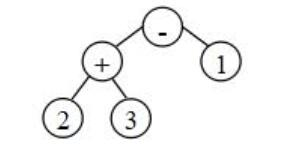
\includegraphics[width=0.6\linewidth]{sampleExpressionTree.jpg}
		\label{sampleExpressionTree}
	\end{figure}\par
	

	\section{设计思路}
	\subsection{二叉树的创建与遍历}
	\textbf{1.构建}\par
	对于这样给出的层序遍历输入,可以按照如下算法来完成建树。为方便理解,使用流程图来描述:\par
	\begin{figure}[H]
		\centering
		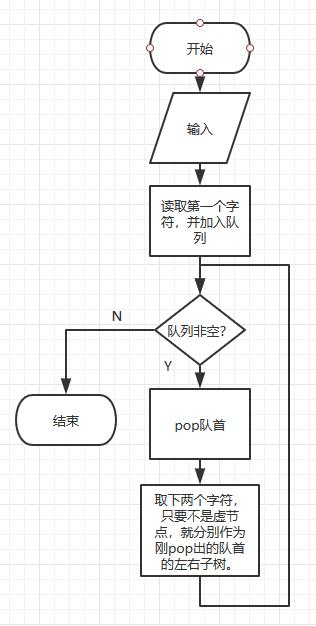
\includegraphics[width=0.6\linewidth]{process1.jpg}
		\label{process1}
	\end{figure}\par

	\textbf{2.后序线索化}\par
	后序线索化的方法主要是按以下几点来进行的:\par
	$\bullet$用pre来记录上一个遍历的结点\par
	$\bullet$递归过程中,首先对左子树递归,再对右子树递归。\par
	$\bullet$其后若本节点左子树指向空,则将本结点的左子树设置为pre;若pre的右子树指向空,则将pre的右子树置为当前节点。\par
	
	\textbf{3.后序线索化后的后序遍历}\par
	对于二叉树的后序线索化的遍历,需要添加双亲节点指针,构建三叉链表才能完成。\par
	后序线索化遍历的过程主要以下面几个准则来进行:\par
	$\bullet$若结点的右子树指向后继结点,则可以直接进行访问\par
	$\bullet$若结点的右子树不指向后继结点,则后继结点应为“对其双亲节点的右子树作后序遍历的第一个结点”\par
	
	\textbf{4.先序遍历与中序遍历}\par
	采用递归遍历,较为简单,故不做赘述。\par
	
	
	\subsection{表达式树}
	\textbf{1.构建}\par
	可以按照如下算法来完成建树。为方便理解,使用流程图来描述:\par
	\begin{figure}[H]
		\centering
		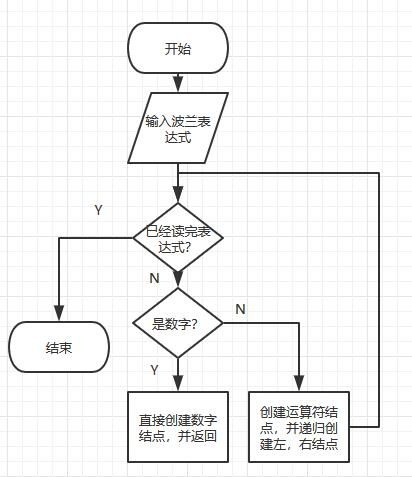
\includegraphics[width=0.6\linewidth]{process2.jpg}
		\label{process2}
	\end{figure}\par
	
	\textbf{2.输出波兰表达式或逆波兰表达式}\par
	只需要对表达式树进行先序遍历或后序遍历即可完成,较为简单,故不赘述。\par
	
	\textbf{3.输出中缀表达式}\par
	主要思路是中序遍历表达式。但值得注意的是怎么确保不加多余的括号。\par
	如果当前结点是'*'或'/',则查看左右结点是否为'+'或'-',如果是,则输出时加上括号;如果不是则不必。\par
	
	\textbf{4.由逆波兰表达式构建表达式树}\par
	对输入字符串的遍历改为从后到前,并且先递归构建当前节点,再右子树,再左子树,即可完成。和\textbf{1.构建}中的描述比较类似。
	
	
	\section{关键代码讲解}
	\subsection{二叉树的创建与遍历}
	\textbf{1.数据类型的定义}\par
	\begin{lstlisting}[language=C++]
	class BTreeNode {
	private:
		BTreeNode* pre = nullptr; //前一个遍历的结点
	public:
		static const char IMAGE_NODE = '#'; //表示虚节点的字符
		char data;
		BTreeNode* left = nullptr, * right = nullptr, * parent = nullptr;
		bool LTag, RTag;
		
		//构建一个结点,其中数据为data,左、右、双亲节点为left, right, parent
		BTreeNode(char data, BTreeNode* left, BTreeNode* right, BTreeNode* parent);
		//参数为题述字符串,构建对应树
		BTreeNode(string layerIter);
		//先序遍历
		static void PreOrderTraverse(BTreeNode* t, void function(BTreeNode*));
		//中序遍历
		static void InOrderTraverse(BTreeNode* t, void function(BTreeNode*));
		//后序遍历
		static void PostOrderTraverse(BTreeNode* t, void function(BTreeNode*));
		//后序线索化
		void PostOrderThreading(BTreeNode* t);
		//利用后序线索化的遍历
		void PostOrderThreadingTraverse(void function(BTreeNode*));
	};
	\end{lstlisting}\par
	
	\textbf{2.主要算法}\par
	\begin{lstlisting}[language=C++, name=建树函数]
	//建树函数
	BTreeNode::BTreeNode(string layerIter) : LTag(false), RTag(false) {
		if (layerIter[0] == IMAGE_NODE) {
			data = IMAGE_NODE;
			cout << "Not a tree!" << endl;
		}
		else {
			//先做好根节点
			data = layerIter[0];
			queue<BTreeNode*> lastLayer;
			lastLayer.push(this);
			int nodeNum = 2;
			int index = 1;
			int strlen = layerIter.length();
			//用index逐一访问字符串layerIter
			while (index < strlen) {
				int qSize = lastLayer.size();
				for (int i = 0; i < qSize; i++) {
					BTreeNode* curNode = lastLayer.front();
					lastLayer.pop();
					if (layerIter[index] != IMAGE_NODE) {
						//如果下一个字符不表示虚节点
						curNode->left =
						new BTreeNode(layerIter[index], nullptr, nullptr, curNode);
						lastLayer.push(curNode->left);
					}
					else //否则是虚节点
					curNode->left = nullptr;
					index++;
					if (layerIter[index] != IMAGE_NODE) {
						//如果下一个字符不表示虚节点
						curNode->right =
						new BTreeNode(layerIter[index], nullptr, nullptr, curNode);
						lastLayer.push(curNode->right);
					}
					else //否则是虚节点
					curNode->right = nullptr;
					index++;
				}
			}
		}
	};
	\end{lstlisting}\par
	\jumpLine
	\begin{lstlisting}[language=C++, name=后序线索化函数]
	//后序线索化函数
	void BTreeNode::PostOrderThreading(BTreeNode* t) {
		if (t == nullptr)
		return;
		//对左子树线索化
		PostOrderThreading(t->left);
		//对右子树线索化
		PostOrderThreading(t->right);
		//对本结点和pre线索化
		if (t->left == nullptr) {
			t->left = pre;
			t->LTag = true;
		}
		if (pre != nullptr && pre->right == nullptr) {
			pre->RTag = true;
			pre->right = t;
		}
		pre = t;
	}
	\end{lstlisting}\par
	\jumpLine
	\begin{lstlisting}[language=C++, name=后序线索化后的遍历函数及启动函数]
	//后序线索化后的遍历函数
	void BTreeNode::PostThreadingTraverse(void function(BTreeNode*)) {
		BTreeNode* temp = this;
		// 找后序遍历的第一个结点
		while (!temp->LTag || !temp->RTag) {
			while (!temp->LTag)
			temp = temp->left;
			while (!temp->RTag)
			temp = temp->right;
		}
		function(temp);
		
		while (temp != nullptr && temp->parent != nullptr) {
			//如果该结点是双亲结点的右孩子或双亲节点没有右孩子
			if (temp->parent->right == temp
			|| temp->parent->RTag) {
				temp = temp->parent;
			}
			else {
				//否则后继结点是双亲节点的右子树中后序遍历第一个结点
				temp = temp->parent->right;
				// 找后序遍历的第一个结点
				while (!temp->LTag || !temp->RTag) {
					while (!temp->LTag)
					temp = temp->left;
					while (!temp->RTag)
					temp = temp->right;
				}
			}
			function(temp);
		}
	}
	
	
	//启动函数
	void BTreeNode::PostOrderThreading(BTreeNode* t) {
		PostThreading(t);
		if (pre != nullptr && pre->right == nullptr) {
			pre->RTag = true;
			pre->right = t;
		}
	}
	\end{lstlisting}\par
	
	\subsection{表达式树}
	\textbf{1.数据类型的定义}\par
	\begin{lstlisting}[language=C++, name=表达式树数据类型定义]
	class ExpressionTree {
		private:
		//由波兰表达式建树
		ExpressionTree* createTree_P(stringstream& ss, ExpressionTree* t);
		//由逆波兰表达式建树
		ExpressionTree* createTree_IP(stringstream& ss, ExpressionTree* t);
		public:
		string op = IMAGE_NODE; //结点的运算符(若为运算符)
		string operand; //结点的数值(若为数)
		bool isOperand = false;
		ExpressionTree* left = nullptr, * right = nullptr;
		const string IMAGE_NODE = "#";
		bool isValueGetted = false;
		int value; //子树值
		
		//通过data和是否是操作数来创建一个结点
		ExpressionTree(string data, bool isOperand);
		//by为1则通过波兰表达式建树,by为0则通过逆波兰表达式建树
		ExpressionTree(string polish, int by);
		
		//打印中缀表达式
		static void printInfixExpression(ExpressionTree* t);
		//打印波兰表达式
		static void printPolishExpression(ExpressionTree* t);
		//打印逆波兰表达式
		static void printInversePolishExpression(ExpressionTree* t);
		//计算各子树的值
		static int getValue(ExpressionTree* t);
	};
	\end{lstlisting}\par
	\textbf{2.主要算法}\par
	思路和前述流程图一样,故不赘述。
	\begin{lstlisting}[language=C++, name=通过波兰表达式建树]
	ExpressionTree* ExpressionTree::createTree_P(stringstream& ss, ExpressionTree* t) {
		string polish;
		ss >> polish;
		if (polish[0] == '+' || polish[0] == '-'
		|| polish[0] == '*' || polish[0] == '/') {
			if (t != this)
			t = new ExpressionTree(polish, false);
			else {
				t->isOperand = false;
				t->isValueGetted = false;
				t->op = polish[0];
			}
			if (!ss.eof()) {
				t->left = createTree_P(ss, t->left);
				t->right = createTree_P(ss, t->right);
			}
		}
		else {
			t = new ExpressionTree(polish, true);
		}
		return t;
	}
	\end{lstlisting}\par
	\jumpLine
	\begin{lstlisting}[language=C++, name=输出中缀表达式的函数]
	void ExpressionTree::printInfixExpression(ExpressionTree* t) {
		if (t != nullptr) {
			//处理左子树
			if (t->left->isOperand) {
				cout << t->left->operand;
			}
			else {
				if ((t->left->op == "+" || t->left->op == "-")
				&& (t->op == "*" || t->op == "/")) {
					cout << '(';
					printInfixExpression(t->left);
					cout << ')';
				}
				else
				printInfixExpression(t->left);
			}
			
			//处理当前结点
			if (t->isOperand) {
				cout << t->operand;
			}
			else {
				cout << t->op;
			}
			
			//处理右子树
			if (t->right->isOperand) {
				cout << t->right->operand;
			}
			else {
				if ((t->right->op == "+" || t->right->op == "-")
				&& (t->op == "*" || t->op == "/")) {
					cout << '(';
					printInfixExpression(t->right);
					cout << ')';
				}
				else
				printInfixExpression(t->right);
			}
		}
	}
	\end{lstlisting}\par
	\jumpLine
	\begin{lstlisting}[language=C++, name=计算表达式树值]
	int ExpressionTree::getValue(ExpressionTree* t) {
		if (t->isValueGetted)
		return t->value;
		else {
			if (t->op == "+") {
				t->value = getValue(t->left) + getValue(t->right);
				t->isValueGetted = true;
				return t->value;
			}
			else if (t->op == "-") {
				t->value = getValue(t->left) - getValue(t->right);
				t->isValueGetted = true;
				return t->value;
			}
			else if (t->op == "*") {
				t->value = getValue(t->left) * getValue(t->right);
				t->isValueGetted = true;
				return t->value;
			}
			else if (t->op == "/") {
				t->value = getValue(t->left) / getValue(t->right);
				t->isValueGetted = true;
				return t->value;
			}
		}
	}
	\end{lstlisting}\par
	
	
	\section{调试分析}
	\subsection{二叉树的创建与遍历}
	\textbf{问题发现与解决}\par
	实验过程中发现自己对于线索二叉树不甚熟悉,翻查各方资料后方能较好地完成线索化。\par
	\textbf{算法的时间复杂度分析}\par
	不论是建树还是遍历,均几乎只访问各个结点一次,时间复杂度接近o(n).\par
	
	\subsection{表达式树}
	\textbf{问题发现与解决}\par
	有了前一个实验的基础,本实验做起来比较简单,没有什么大问题。\par
	\textbf{算法的时间复杂度分析}\par
	同样的,各个结点均几乎只访问一次,时间复杂度接近o(n).\par
	
	
	\section{代码测试}
	\subsection{二叉树的创建与遍历}
	\textbf{输入1:}\par
	\fbox{
		\parbox{0.8\linewidth}{
			AB\#C\#D\#\#E\#\#\\
		}
	}\par
	\textbf{输出截图1:}\par
	\begin{figure}[H]
		\centering
		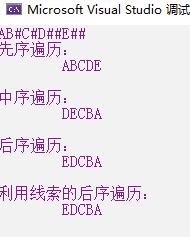
\includegraphics[width=0.5\linewidth]{test1_1.jpg}
		\label{test1_1}
	\end{figure}\par
	\jumpLine
	\textbf{输入2:}\par
	\fbox{
		\parbox{0.8\linewidth}{
			A\#BC\#\#DE\#\#F\#\#\\
		}
	}\par
	\textbf{输出截图2:}\par
	\begin{figure}[H]
		\centering
		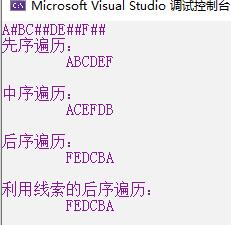
\includegraphics[width=0.5\linewidth]{test1_2.jpg}
		\label{test1_2}
	\end{figure}\par
	\jumpLine
	\textbf{输入3:}\par
	\fbox{
		\parbox{0.8\linewidth}{
			ABCD\#\#E\#\#F\#\#\#\\
		}
	}\par
	\textbf{输出截图3:}\par
	\begin{figure}[H]
		\centering
		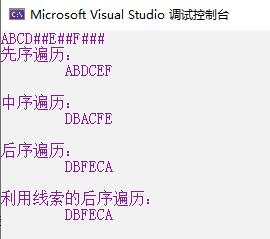
\includegraphics[width=0.5\linewidth]{test1_3.jpg}
		\label{test1_3}
	\end{figure}\par

	\subsection{表达式树}
	\textbf{输入1:}\par
	\fbox{
		\parbox{0.8\linewidth}{
			+ 2 * 30 5\\
		}
	}\par
	\textbf{输出截图1:}\par
	\begin{figure}[H]
		\centering
		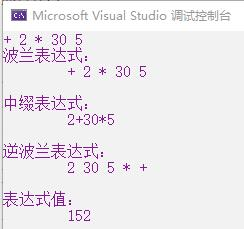
\includegraphics[width=0.5\linewidth]{test2_1.jpg}
		\label{test2_1}
	\end{figure}\par
	\jumpLine
	\textbf{输入2:}\par
	\fbox{
		\parbox{0.8\linewidth}{
			/ + 15 * 5 + 2 18 5\\
		}
	}\par
	\textbf{输出截图2:}\par
	\begin{figure}[H]
		\centering
		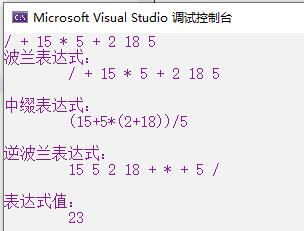
\includegraphics[width=0.5\linewidth]{test2_2.jpg}
		\label{test2_2}
	\end{figure}\par
	\jumpLine
	\textbf{输入3:}\par
	\fbox{
		\parbox{0.8\linewidth}{
			- / 15 - 2 7 10\\
		}
	}\par
	\textbf{输出截图3:}\par
	\begin{figure}[H]
		\centering
		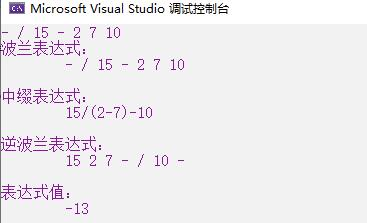
\includegraphics[width=0.5\linewidth]{test2_3.jpg}
		\label{test2_3}
	\end{figure}\par



	\section{实验总结}
	首先回答几个思考题。\par
	\textbf{1.}给定先序和中序序列、中序和后序序列、先序和后序序列均可以唯一确定一棵树。\par
	$\bullet$先序+中序:逐一遍历先序序列的结点,对当前遍历的结点,在中序序列中可以知道其左右子树中的结点(在该结点左边就是左子树结点,右边就是右子树结点),如此递归即可确定下一棵树。\par
	$\bullet$中序+后序:逐一遍历后序序列的结点,类似于“先序+中序”的情况,也可以解决。\par
	$\bullet$先序+后序:逐一遍历先序序列中的结点,可以其剩余序列分为左子树和右子树,同理在后序序列中找到该结点,其前面的序列也分为该节点的左子树和右子树。只需找到对应长度的序列,即可确定该节点的左右子树,从而递归地完成建树。\par
	\textbf{2.}表达式树的先序序列对应波兰表达式;中序序列不考虑括号则对应中缀表达式是;后序序列对应逆波兰表达式。\par
	\textbf{3.}给定波兰式、中缀表达式或逆波兰式中的任意一种,可以唯一确定一颗表达式树。造成这种差异的原因是:表达式树的叶子只能是数值,数值也只能在叶子上,而符号则在分支上。这样就给出了足够多的约束条件。\par
	\jumpLine\par
	本次实验让我深刻了解了二叉树的创建,线索化,及线索化遍历。此外,还以此为基础,完成了表达式树的一些操作。虽然实验任务量相对较大,但学到的东西也更多。\par
	
	
	
	
	
	
	
	\section{附录}
	\subsection{附录A.二叉树的创建与遍历}
	\begin{lstlisting}[language=C++, name=BTreeNode.h]
	#include <iostream>
	#include <string>
	#include <queue>
	#pragma once
	
	using namespace std;
	
	class BTreeNode {
		private:
		BTreeNode* pre = nullptr; //前一个遍历的结点
		public:
		static const char IMAGE_NODE = '#'; //表示虚节点的字符
		char data;
		BTreeNode* left = nullptr, * right = nullptr, * parent = nullptr;
		bool LTag, RTag;
		
		//构建一个结点,其中数据为data,左、右、双亲节点为left, right, parent
		BTreeNode(char data, BTreeNode* left, BTreeNode* right, BTreeNode* parent);
		//参数为题述字符串,构建对应树
		BTreeNode(string layerIter);
		//先序遍历
		static void PreOrderTraverse(BTreeNode* t, void function(BTreeNode*));
		//中序遍历
		static void InOrderTraverse(BTreeNode* t, void function(BTreeNode*));
		//后序遍历
		static void PostOrderTraverse(BTreeNode* t, void function(BTreeNode*));
		//后序线索化子程序
		void PostThreading(BTreeNode* t);
		//后序线索化
		void PostOrderThreading(BTreeNode* t);
		//利用后序线索化的遍历
		void PostOrderThreadingTraverse(void function(BTreeNode*));
	};
	
	
	BTreeNode::BTreeNode(char data, BTreeNode* left, BTreeNode* right, BTreeNode* parent)
	: data(data), left(left), right(right), parent(parent),
	LTag(false), RTag(false) {};
	
	BTreeNode::BTreeNode(string layerIter) : LTag(false), RTag(false) {
		if (layerIter[0] == IMAGE_NODE) {
			data = IMAGE_NODE;
			cout << "Not a tree!" << endl;
		}
		else {
			//先做好根节点
			data = layerIter[0];
			queue<BTreeNode*> lastLayer;
			lastLayer.push(this);
			int nodeNum = 2;
			int index = 1;
			int strlen = layerIter.length();
			//用index逐一访问字符串layerIter
			while (index < strlen) {
				int qSize = lastLayer.size();
				for (int i = 0; i < qSize; i++) {
					BTreeNode* curNode = lastLayer.front();
					lastLayer.pop();
					if (layerIter[index] != IMAGE_NODE) {
						//如果下一个字符不表示虚节点
						curNode->left =
						new BTreeNode(layerIter[index], nullptr, nullptr, curNode);
						lastLayer.push(curNode->left);
					}
					else //否则是虚节点
					curNode->left = nullptr;
					index++;
					if (layerIter[index] != IMAGE_NODE) {
						//如果下一个字符不表示虚节点
						curNode->right =
						new BTreeNode(layerIter[index], nullptr, nullptr, curNode);
						lastLayer.push(curNode->right);
					}
					else //否则是虚节点
					curNode->right = nullptr;
					index++;
				}
			}
		}
	};
	
	void BTreeNode::PreOrderTraverse(BTreeNode* t, void function(BTreeNode*)) {
		if (t != nullptr)
		{
			function(t);
			if (t->LTag == 0)
			PreOrderTraverse(t->left, function);
			if (t->RTag == 0)
			PreOrderTraverse(t->right, function);
		}
	}
	
	void BTreeNode::InOrderTraverse(BTreeNode* t, void function(BTreeNode*)) {
		if (t != nullptr)
		{
			if (t->LTag == 0)
			InOrderTraverse(t->left, function);
			function(t);
			if (t->RTag == 0)
			InOrderTraverse(t->right, function);
		}
	}
	
	void BTreeNode::PostOrderTraverse(BTreeNode* t, void function(BTreeNode*)) {
		if (t != nullptr)
		{
			if (t->LTag == 0)
			PostOrderTraverse(t->left, function);
			if (t->RTag == 0)
			PostOrderTraverse(t->right, function);
			function(t);
		}
	}
	
	void BTreeNode::PostThreading(BTreeNode* t) {
		if (t == nullptr)
		return;
		//对左子树线索化
		PostThreading(t->left);
		//对右子树线索化
		PostThreading(t->right);
		//对本结点和pre线索化
		if (t->left == nullptr) {
			t->left = pre;
			t->LTag = true;
		}
		if (pre != nullptr && pre->right == nullptr) {
			pre->RTag = true;
			pre->right = t;
		}
		pre = t;
	}
	
	void BTreeNode::PostOrderThreading(BTreeNode* t) {
		PostThreading(t);
		if (pre != nullptr && pre->right == nullptr) {
			pre->RTag = true;
			pre->right = t;
		}
	}
	
	void BTreeNode::PostOrderThreadingTraverse(void function(BTreeNode*)) {
		BTreeNode* temp = this;
		// 找后序遍历的第一个结点
		while (!temp->LTag || !temp->RTag) {
			while (!temp->LTag)
			temp = temp->left;
			while (!temp->RTag)
			temp = temp->right;
		}
		function(temp);
		
		while (temp != nullptr && temp->parent != nullptr) {
			//如果该结点是双亲结点的右孩子或双亲节点没有右孩子
			if (temp->parent->right == temp
			|| temp->parent->RTag) {
				temp = temp->parent;
			}
			else {
				//否则后继结点是双亲节点的右子树中后序遍历第一个结点
				temp = temp->parent->right;
				// 找后序遍历的第一个结点
				while (!temp->LTag || !temp->RTag) {
					while (!temp->LTag)
					temp = temp->left;
					while (!temp->RTag)
					temp = temp->right;
				}
			}
			function(temp);
		}
	}
	\end{lstlisting}
	\jumpLine
	\begin{lstlisting}[language=C++, name=二叉树的创建与遍历main.c]
	#include <iostream>
	#include "BTreeNode.h"
	using namespace std;
	
	void printTree(BTreeNode* t)
	{
		if(t != nullptr)
		cout << t->data;
	}
	
	int main()
	{
		BTreeNode* t = &BTreeNode("ABC#DEFG##H######");
		BTreeNode::PreOrderTraverse(t, printTree);
		cout << endl;
		BTreeNode::InOrderTraverse(t, printTree);
		cout << endl;
		BTreeNode::PostOrderTraverse(t, printTree);
		cout << endl;
		t->PostOrderThreading(t);
		t->PostOrderThreadingTraverse(printTree);
	}
	\end{lstlisting}
	
	
	\subsection{附录B.表达式树}
	\begin{lstlisting}[language=C++, name=ExpressionTree.h]
	#include <iostream>
	#include <string>
	#include <queue>
	#include <cstring>
	#pragma once
	
	using namespace std;
	
	class ExpressionTree {
		private:
		//由波兰表达式建树
		ExpressionTree* createTree_P(stringstream& ss, ExpressionTree* t);
		//由逆波兰表达式建树
		ExpressionTree* createTree_IP(stringstream& ss, ExpressionTree* t);
		public:
		string op = IMAGE_NODE; //结点的运算符(若为运算符)
		string operand; //结点的数值(若为数)
		bool isOperand = false;
		ExpressionTree* left = nullptr, * right = nullptr;
		const string IMAGE_NODE = "#";
		bool isValueGetted = false;
		int value; //子树值
		
		//通过data和是否是操作数来创建一个结点
		ExpressionTree(string data, bool isOperand);
		//by为1则通过波兰表达式建树,by为0则通过逆波兰表达式建树
		ExpressionTree(string polish, int by);
		
		//打印中缀表达式
		static void printInfixExpression(ExpressionTree* t);
		//打印波兰表达式
		static void printPolishExpression(ExpressionTree* t);
		//打印逆波兰表达式
		static void printInversePolishExpression(ExpressionTree* t);
		//计算各子树的值
		static int getValue(ExpressionTree* t);
	};
	
	ExpressionTree::ExpressionTree(string data, bool isOperand) {
		this->isOperand = isOperand;
		if (isOperand) {
			operand = data;
			stringstream ss(data);
			ss >> value;
			isValueGetted = true;
		}
		else {
			isValueGetted = false;
			op = data[0];
		}
	}
	
	ExpressionTree* ExpressionTree::createTree_P(stringstream& ss, ExpressionTree* t) {
		string polish;
		ss >> polish;
		if (polish[0] == '+' || polish[0] == '-'
		|| polish[0] == '*' || polish[0] == '/') {
			if (t != this)
			t = new ExpressionTree(polish, false);
			else {
				t->isOperand = false;
				t->isValueGetted = false;
				t->op = polish[0];
			}
			if (!ss.eof()) {
				t->left = createTree_P(ss, t->left);
				t->right = createTree_P(ss, t->right);
			}
		}
		else {
			t = new ExpressionTree(polish, true);
		}
		return t;
	}
	
	ExpressionTree* ExpressionTree::createTree_IP(stringstream& ss, ExpressionTree* t) {
		string polish;
		ss >> polish;
		if (polish[0] == '+' || polish[0] == '-'
		|| polish[0] == '*' || polish[0] == '/') {
			if (t != this)
			t = new ExpressionTree(polish, false);
			else {
				t->isOperand = false;
				t->isValueGetted = false;
				t->op = polish[0];
			}
			if (!ss.eof()) {
				t->right = createTree_IP(ss, t->right);
				t->left = createTree_IP(ss, t->left);
			}
		}
		else {
			t = new ExpressionTree(polish, true);
		}
		return t;
	}
	
	ExpressionTree::ExpressionTree(string polish, int by) {
		if (by) {
			stringstream ss(polish);
			createTree_P(ss, this);
		}
		else {
			int len = polish.length();
			stringstream ss(polish);
			string inversed;
			while (!ss.eof()) {
				string temp;
				ss >> temp;
				inversed = temp + " " + inversed;
			}
			stringstream iss(inversed);
			createTree_IP(iss, this);
		}
	}
	
	void ExpressionTree::printInfixExpression(ExpressionTree* t) {
		if (t != nullptr) {
			//处理左子树
			if (t->left->isOperand) {
				cout << t->left->operand;
			}
			else {
				if ((t->left->op == "+" || t->left->op == "-")
				&& (t->op == "*" || t->op == "/")) {
					cout << '(';
					printInfixExpression(t->left);
					cout << ')';
				}
				else
				printInfixExpression(t->left);
			}
			
			//处理当前结点
			if (t->isOperand) {
				cout << t->operand;
			}
			else {
				cout << t->op;
			}
			
			//处理右子树
			if (t->right->isOperand) {
				cout << t->right->operand;
			}
			else {
				if ((t->right->op == "+" || t->right->op == "-")
				&& (t->op == "*" || t->op == "/")) {
					cout << '(';
					printInfixExpression(t->right);
					cout << ')';
				}
				else
				printInfixExpression(t->right);
			}
		}
	}
	
	void ExpressionTree::printPolishExpression(ExpressionTree* t)
	{
		if (t != nullptr) {
			if (t->isOperand)
			cout << t->operand << ' ';
			else
			cout << t->op << ' ';
			printPolishExpression(t->left);
			printPolishExpression(t->right);
		}
	}
	
	void ExpressionTree::printInversePolishExpression(ExpressionTree* t)
	{
		if (t != nullptr) {
			printInversePolishExpression(t->left);
			printInversePolishExpression(t->right);
			if (t->isOperand)
			cout << t->operand << ' ';
			else
			cout << t->op << ' ';
		}
	}
	
	int ExpressionTree::getValue(ExpressionTree* t) {
		if (t->isValueGetted)
		return t->value;
		else {
			if (t->op == "+") {
				t->value = getValue(t->left) + getValue(t->right);
				t->isValueGetted = true;
				return t->value;
			}
			else if (t->op == "-") {
				t->value = getValue(t->left) - getValue(t->right);
				t->isValueGetted = true;
				return t->value;
			}
			else if (t->op == "*") {
				t->value = getValue(t->left) * getValue(t->right);
				t->isValueGetted = true;
				return t->value;
			}
			else if (t->op == "/") {
				t->value = getValue(t->left) / getValue(t->right);
				t->isValueGetted = true;
				return t->value;
			}
		}
	}
	\end{lstlisting}
	
	
\end{document}
